\documentclass[12pt, a4paper, twoside]{scrartcl}

\renewcommand{\familydefault}{\sfdefault}

\usepackage{siunitx, pdfpages}
\usepackage[europeanresistors, americaninductors]{circuitikz}
\usetikzlibrary{arrows.meta}
\usepackage{mystyle}

\newcommand{\LTI}[4][1]{
  \begin{center}
    \begin{tikzpicture}[scale=#1]
      \draw[->, thick] (0,1) -- (2,1);
      \draw[thick] (2,0) rectangle (5,2) node [pos=.5] {#3};
      \draw[->, thick] (5,1) -- (7,1);
      \draw [above] (0,1) node {#2};
      \draw [above] (7,1) node {#4};
      \draw [above] (3.5,2) node {\sffamily LTI};
    \end{tikzpicture}
  \end{center}
}

\usepackage{scrlayer-scrpage}

\clearpairofpagestyles{}

\setkomafont{pageheadfoot}{\sffamily\footnotesize}
\setkomafont{pagination}{}

\ohead{Seite~\pagemark}
\ihead{Tim Hilt}

\KOMAoptions{
  headsepline=true,
}

\title{Formelsammlung --- Signale und Systeme}
\subtitle{bei Prof.\ Thao Dang}
\author{Tim Hilt}
\date{\today}

\begin{document}

\maketitle
\tableofcontents
\clearpage

\section{Grundlagen und Metriken}

\textbf{Eigenschaften Allgemeine Cosinusfunktion}
\begin{align*}
  f(t) &= A\cos(\omega \cdot t + \varphi)\\
  T &= \frac{2\pi}{\omega} \quad ; \quad \omega = \frac{2\pi}{T}
\end{align*}

\textbf{Betrag einer komplexen Zahl}
\begin{align*}
  Z &= x+ jy\\
  |Z| &= \sqrt{x^2 +y^2}
\end{align*}

\textbf{Winkel einer komplexen Zahl}
\[\arg (Z) = \varphi =
  \begin{cases}
    \arctan \left(\frac{y}{x}\right) & \text{für } x>0, y \text{ bel.}\\
    \arctan \left(\frac{y}{x}\right) + \pi & \text{für } x<0, y \text{ bel.}\\
    \frac{\pi}{2} & \text{für } x = 0, y > 0\\
    - \frac{\pi}{2} & \text{für } x = 0,y < 0
  \end{cases}\]

\textbf{Dämpfung zweier Pegel}
\begin{align*}
  a &= 20 \cdot \log \left(\frac{\text{Eingang}}{\text{Ausgang}} \right) \si{\decibel}\\
  \intertext{und wenn Eingang = 1:}
  &= -20 \cdot \log(\textrm{Ausgang}) \si{\decibel}
\end{align*}

\textbf{Phasengang}
\[b(f) = -\arg(Z)\]
Die Phase muss dem negativen Winkel entsprechen, um bei nachlaufendem Signal eine positive Zeitverzögerung zu erhalten.

\textbf{Phasenlaufzeit/Zeitverzögerung}
\[t_p = \frac{b(f)}{\omega}\]

\clearpage
\section{LTI-Systeme}

\begin{figure}[H]
  \centering
  \begin{circuitikz}
    \draw[very thick] (0,0) node [ocirc]{} -- (1.5,0);
    \draw[very thick] (4.5,0) -- (6,0) node [ocirc]{};
    \draw[very thick] (0,-2) node [ocirc]{} -- (1.5,-2);
    \draw[very thick] (4.5,-2) -- (6,-2) node [ocirc]{};
    \draw[] (-.5,0) to [open, v=\(U_e\)] (-.5, -2);
    \draw[] (6.5,0) to [open, v^=\(U_a\)] (6.5, -2);
    \draw[very thick] (1.5,.25) rectangle (4.5,-2.25) node [pos=.5]{\huge\sffamily LTI};
    \draw (0,-3) node {\(x(t)\)};
    \draw (1.5,-3) node {\(\star\)};
    \draw (3,-3) node {\(h(t)\)};
    \draw (4.5,-3) node {\(=\)};
    \draw (6,-3) node {\(y(t)\)};

    \draw (0,-4) node {\(X(p)\)};
    \draw (1.5,-4) node {\(\cdot\)};
    \draw (3,-4) node {\(H(p)\)};
    \draw (4.5,-4) node {\(=\)};
    \draw (6,-4) node {\(Y(p)\)};
  \end{circuitikz}
  \caption{LTI-System}
\end{figure}

\textbf{Linearität}\\
Ein System gilt als linear, \mytextcol{wenn zum Signal nichts addiert wird}, sondern dass Signal nur entweder verschoben entlang der \(t\)-Achse oder skaliert in \(y\)-Richtung ist.

\textbf{Zeitinvarianz}\\
Wird das Signal \(x(t)\) noch \mytextcol{mit einer anderen Funktion, die von \(t\) abhängt multipliziert}, dann ist das System \mybfcol{nicht} zeitinvariant, da diese Funktion sich mit der Zeit verändert und \(x(t)\) somit immer mit anderen Werten multipliziert wird.

Bsp.:

\begin{center}
  \begin{tabular}{ll}
    \(y(t) = \sqrt{2}x(t)\) & \mytextcol{zeitinvariant}\\
    \(y(t) = x(t) \cdot \sin(t)\) & \mytextcol{zeitvariant!}\\
    \(y(t) = x^2(t)\) & \mytextcol{auch zeitvariant}
  \end{tabular}
\end{center}


\textbf{Kausalität}\\
Ein Signal ist kausal, \mytextcol{wenn gilt \(x(t) = 0\) für \(t < 0\)}

\textbf{Stabilität}\\
Beim Betrachten der Stabilität unterscheidet man 3 Fälle:
\begin{enumerate}
\item \mytextcol{Das System ist stabil}, wenn alle Pole im Pol-Nullstellen-Diagramm in der linken Halbebene liegen
\item \mytextcol{Das System ist grenzstabil}, wenn nur einfache Pole im Pol-Nullstellen-Diagramm auf der imaginären Achse liegen
\item \mytextcol{Das System ist instabil}, wenn Pole in der rechten Halbebene des Pol-Nullstellen-Diagramms liegen und/oder mehrfache Pole auf der imaginären Achse liegen
\end{enumerate}
\newpage
\textbf{Sprungantwort und Impulsantwort}

Die Sprungantwort ist das Ausgangssignal eines Systems wenn am Eingang die Sprungfunktion \(\sigma(t)\) angelegt wird. Sie wird allgemein auch mit \mytextcol{\(a(t)\)} bezeichnet.

\LTI[.5]{\(\sigma(t)\)}{\(h(t)\)}{\(a(t)\)}

Die Impulsantwort hingegen ist das Ausgangssignal eines Systems, wenn am Eingang die Impulsfunktion \(\delta(t)\) angelegt wird. Sie wird allgemein auch mit \mytextcol{\(h(t)\)} bezeichnet.

\LTI[.5]{\(\delta(t)\)}{\(h(t)\)}{\(h(t)\)}

Um von der Sprungantwort auf die Impulsantwort zu schließen muss \mybfcol{Die Sprungantwort einmal abgeleitet werden,} da gilt:
\[\sigma(t)' = \delta(t) \quad\Longleftrightarrow\quad a(t)' = h(t)\]
Demnach gilt auch:
\[\int h(t) dt = a(t)\]

\clearpage
\section{Fourierreihen}

\[f(t) = \frac{a_0}{2} + \sum_{k=1}^{\infty}(a_k \cos (k \omega t) + b_k \sin (k \omega t)), \quad \omega = \frac{2 \pi}{T}\]

\textbf{Gleichanteil}

\[s_G \quad = \quad \frac{\text{Integral über eine Periode}}{\text{Periodendauer}}\]

\textbf{Reelle Fourier-Koeffizienten \(a_k\) und \(b_k\)}

\begin{align*}
  a_k &= \frac{2}{T} \int_{-\frac{T}{2}}^{\frac{T}{2}}f(t) \cos (k \omega t) dt\\[1em]
  b_k &= \frac{2}{T} \int_{-\frac{T}{2}}^{\frac{T}{2}}f(t) \sin (k \omega t) dt
\end{align*}

\textbf{Umrechnung von \(c_k\) zu \(a_k\) und \(b_k\)}
\begin{empheq}[box = \fbox]{align*}
  a_k &= 2 \mathrm{Re}(c_k)\\[1em]
  b_k &= -2 \mathrm{Im}(c_k)\\[1em]
  \rightarrow c_k &= \frac{a_k-ib_k}{2}
\end{empheq}

\clearpage
\section{Fouriertransformation}

\textbf{Fourierreihe aus Fouriertransformation}\\
\mybfcol{Achtung:} stetiges \(f\) der Fouriertransformation wird durch diskretes \(\frac{k}{T}\) ersetzt
\begin{align*}
  \frac{1}{T} &= f_0\\
  s(t)\quad &\laplace\quad S(f)\\
  c_k &= \frac{1}{T} \cdot S\left(\frac{k}{T}\right)
\end{align*}
Demnach lässt sich der Gleichanteil berechnen durch:
\begin{empheq}[box = \fbox]{align*}
  c_0 = \frac{1}{T} \cdot S\left(\frac{0}{T}\right)
\end{empheq}

\clearpage
\section{Faltung}

\begin{framed}
  Werden zwei Signale \(u_1(t), u_2(t)\)~unterschiedlicher Bandbreiten \(T_1, T_2\)~gefaltet,\\
  so beträgt die Bandbreite des neuen Signals \(T_1 + T_2\).
\end{framed}

\textbf{Faltung mit \(\sigma (t)\)}\\

Wird eine Funktion mit \(\sigma (t)\) gefaltet, so ergibt sich für das Faltungsintegral:

\[n(t) \star \sigma (t) = \int_{-\infty}^{\infty} n(\tau) \cdot \sigma(t - \tau) d\tau = \int_{-\infty}^t n(\tau) d\tau\]

\clearpage
\section{Filter und Übertragungsfunktionen}

Im Fourierbereich: \(\omega = 2 \pi f\), im Laplacebereich: \(j\omega = p\)

{
  \centering
  \begin{tabular}{cllll}
    \toprule
    & \textbf{RC-Tiefpass} & \textbf{RC-Hochpass} & \textbf{RL-Tiefpass} & \textbf{RL-Hochpass}\\
    \midrule
    \textbf{\(\frac{U_a}{U_e} = H(j\omega)\)} & \(\frac{1}{1 + j\omega R C}\) & \(\frac{j\omega RC}{1 + j\omega RC}\) & \(\frac{R}{R + j \omega L}\)& \(\frac{j\omega L}{R + j \omega L}\) \\[1em]
    \textbf{\(f_G / \omega_G\)} & \(\frac{1}{2 \pi R C}; \frac{1}{RC}\) & \(\frac{1}{2 \pi R C}; \frac{1}{RC}\) & \(\frac{R}{2 \pi L}; \frac{R}{L}\) & \(\frac{R}{2 \pi L}; \frac{R}{L}\)\\
    \bottomrule
  \end{tabular}
}

\begin{minipage}{.48\linewidth}
  \begin{figure}[H]
    \centering
    \begin{circuitikz}
      \draw (0,0) to [R, l=\(R\)] (4,0) to [C, l_=\(C\)] (4,-2) node[rground]{};
      \draw (0,0) to [european voltage source] (0,-2) node[rground]{};
      \draw (-.5,0) to [open, v=\(U_e\)] (-.5,-2);
      \draw (4.5,0) to [open, v^=\(U_a\)] (4.5,-2);
    \end{circuitikz}
    \caption{RC-Tiefpass}
  \end{figure}
  \begin{figure}[H]
    \centering
    \begin{circuitikz}
      \draw (0,0) to [L, l=\(L\)] (4,0) to [R, l_=\(R\)] (4,-2) node[rground]{};
      \draw (0,0) to [european voltage source] (0,-2) node[rground]{};
      \draw (-.5,0) to [open, v=\(U_e\)] (-.5,-2);
      \draw (4.5,0) to [open, v^=\(U_a\)] (4.5,-2);
    \end{circuitikz}
    \caption{RL-Tiefpass}
  \end{figure}
\end{minipage}\hfill%
\begin{minipage}{.48\linewidth}
  \begin{figure}[H]
    \centering
    \begin{circuitikz}
      \draw (0,0) to [C, l=\(C\)] (4,0) to [R, l_=\(R\)] (4,-2) node[rground]{};
      \draw (0,0) to [european voltage source] (0,-2) node[rground]{};
      \draw (-.5,0) to [open, v=\(U_e\)] (-.5,-2);
      \draw (4.5,0) to [open, v^=\(U_a\)] (4.5,-2);
    \end{circuitikz}
    \caption{RC-Hochpass}
  \end{figure}
  \begin{figure}[H]
    \centering
    \begin{circuitikz}
      \draw (0,0) to [R, l=\(R\)] (4,0) to [L, l_=\(L\)] (4,-2) node[rground]{};
      \draw (0,0) to [european voltage source] (0,-2) node[rground]{};
      \draw (-.5,0) to [open, v=\(U_e\)] (-.5,-2);
      \draw (4.5,0) to [open, v^=\(U_a\)] (4.5,-2);
    \end{circuitikz}
    \caption{RL-Hochpass}
  \end{figure}
\end{minipage}

\textbf{Kondensator und Spule im Frequenzbereich}

\begin{center}
  \begin{tabular}{lll}
    \toprule
    Frequenz & Spule & Kondensator\\
    \midrule
    \(\SI{0}{\hertz}\) & \(Z_L = \SI{0}{\ohm}\); Kurzschluss & \(Z_C = \infty\ \si{\ohm}\); Leerlauf\\
    \(\infty\ \si{\hertz}\) & \(Z_L = \infty\ \si{\ohm}\); Leerlauf & \(Z_C = \SI{0}{\ohm}\); Kurzschluss\\
    \bottomrule
  \end{tabular}
\end{center}

\clearpage
\section{Konstruktion Bode-Diagramm}

\textbf{Für Pol- Nullstellendiagramm:}

\begin{enumerate}
\item \(p\)s im Nenner und im Zähler isolieren
\item Pol- und Nullstellen für \(p\) finden
\item Polstellen als \(\times\) und Nullstellen als \(\bigcirc\) in ein \(\operatorname{Re} / \operatorname{Im}\)-Diagramm (\(p\)-Ebene) eintragen
\end{enumerate}

\textbf{Bode-Diagramm}

Das Bode-Diagramm besteht aus dem \textbf{Amplitudengang} und dem \textbf{Phasengang}. Der Amplitudengang \(A(f)\) lässt sich berechnen durch
\[A(f) = -20\log(|H(f)|)\]
während sich der Phasengang \(b(f)\) berechnen lässt über
\[b(f) = -\arctan\left(\frac{\operatorname{Im}(H(f))}{\operatorname{Re}(H(f))}\right) +
  \begin{cases}
    0 & \operatorname{Re}(H(f)) > 0\\
    \pm \pi & \operatorname{Re}(H(f)) < 0
  \end{cases}
\]

\textbf{Sprungantwort schnell berechnen}
\[a(t) = (a(0) - a(\infty)) \cdot e^{-\frac{t}{T}} + a(\infty)\]

\newpage
\phantomsection%
\addtocounter{section}{1}
\addsectiontocentry{\arabic{section}}{Anhang}

\newpage
\phantomsection%
\addtocounter{subsection}{1}
\addsubsectiontocentry{A}{Tabellen aus Buch von Prof.\ Koch und Prof.\ Stämpfle}
\includepdf[pages=7-]{Cheatsheet.pdf}

\newpage
\phantomsection%
\addtocounter{subsection}{1}
\addsubsectiontocentry{B}{Tabelle aus Vorlesung}
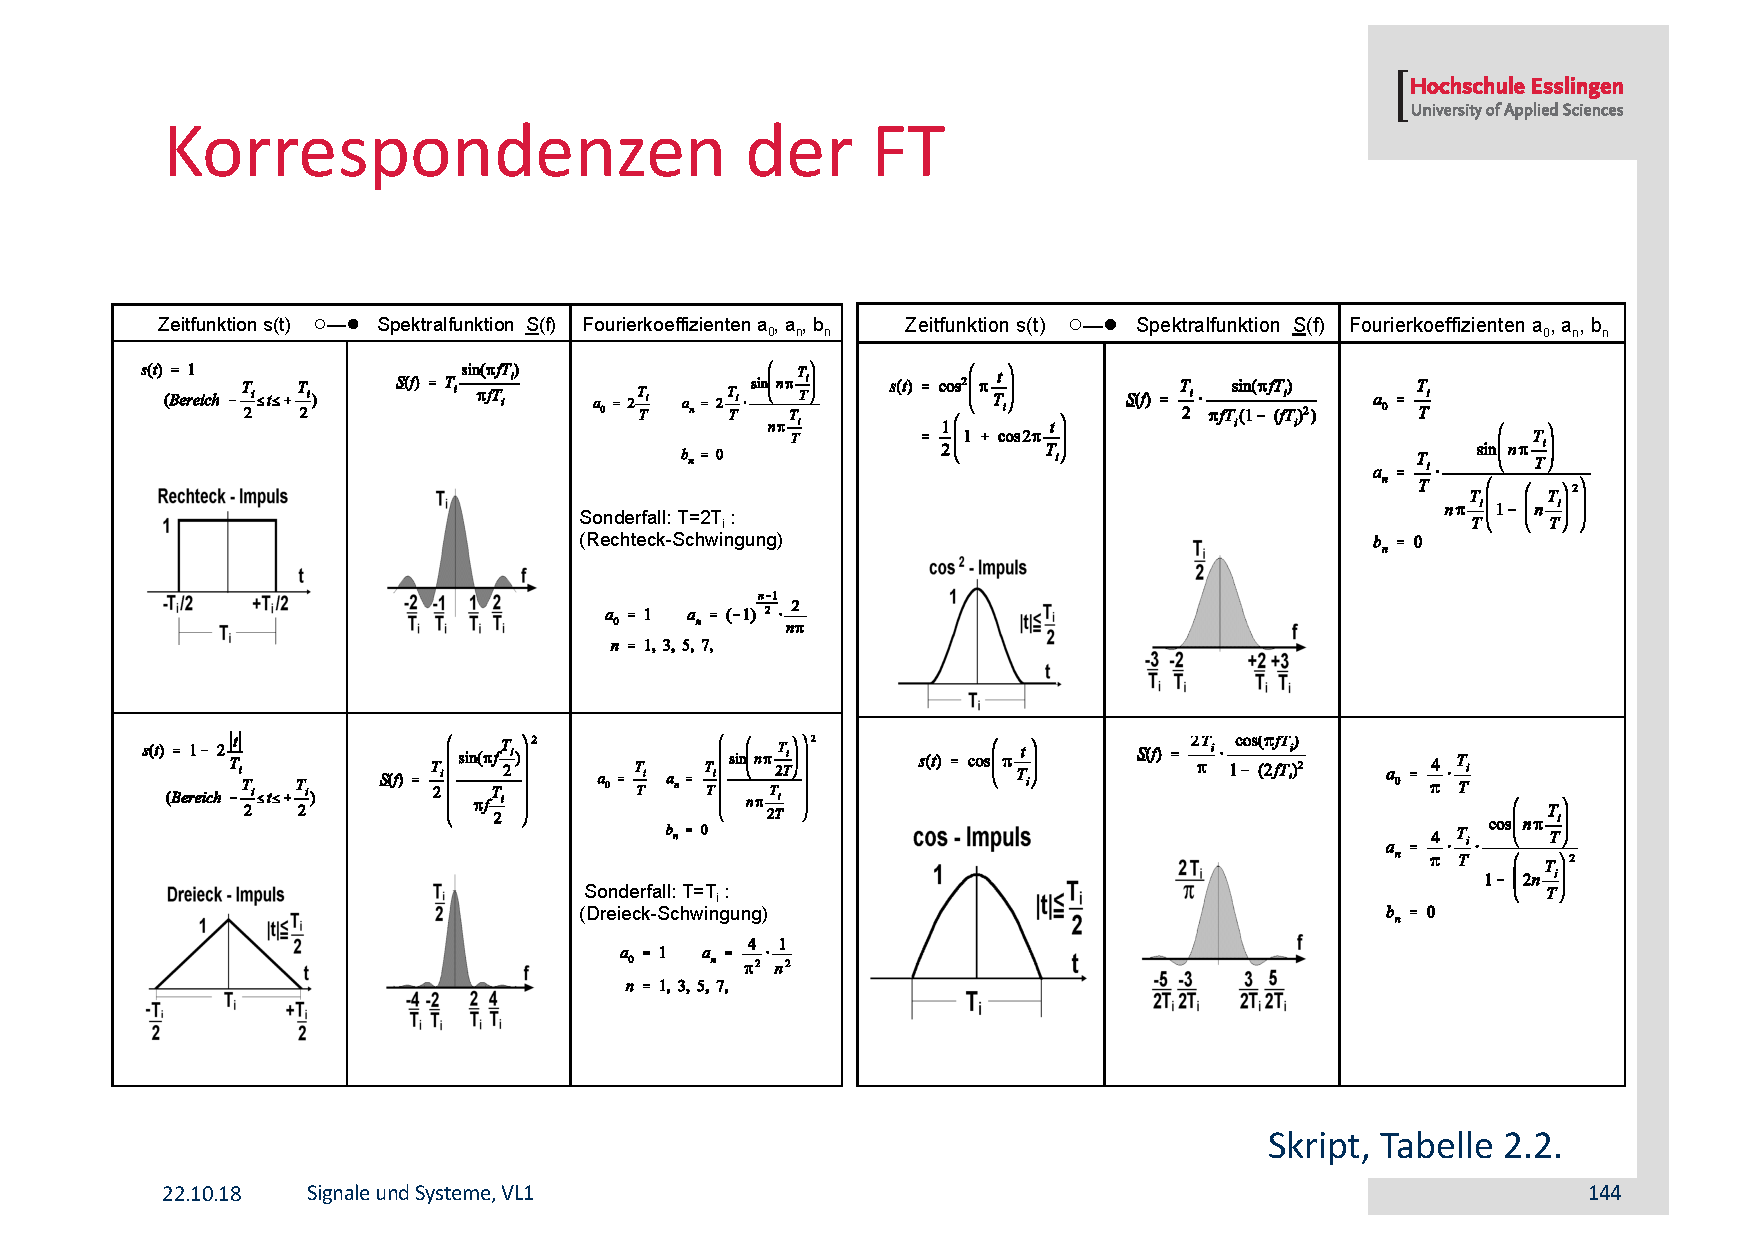
\includepdf{FourierKorrespondenzen.pdf}

\end{document}

%%% Local Variables:
%%% mode: latex
%%% TeX-master: t
%%% End:
